\documentclass[12pt,letterpaper]{article}
\usepackage{amsmath}
\usepackage{tcolorbox}
\usepackage{graphicx}
\graphicspath{{.}}
\usepackage{geometry}


\newcommand{\RomanNumeralCaps}[1]
    {\MakeUppercase{\romannumeral #1}}

\author{Noah Fryer 113387301}
\title{Project 0}

\begin{document}

    \maketitle
    
    \section*{Server Running on gpel8}

    To get this part working, I copied the code from the project specification, changed the port that the client and server were using, and then followed the rest of the directions to run the client and the server on the same machine.

    \vspace{1 cm}

    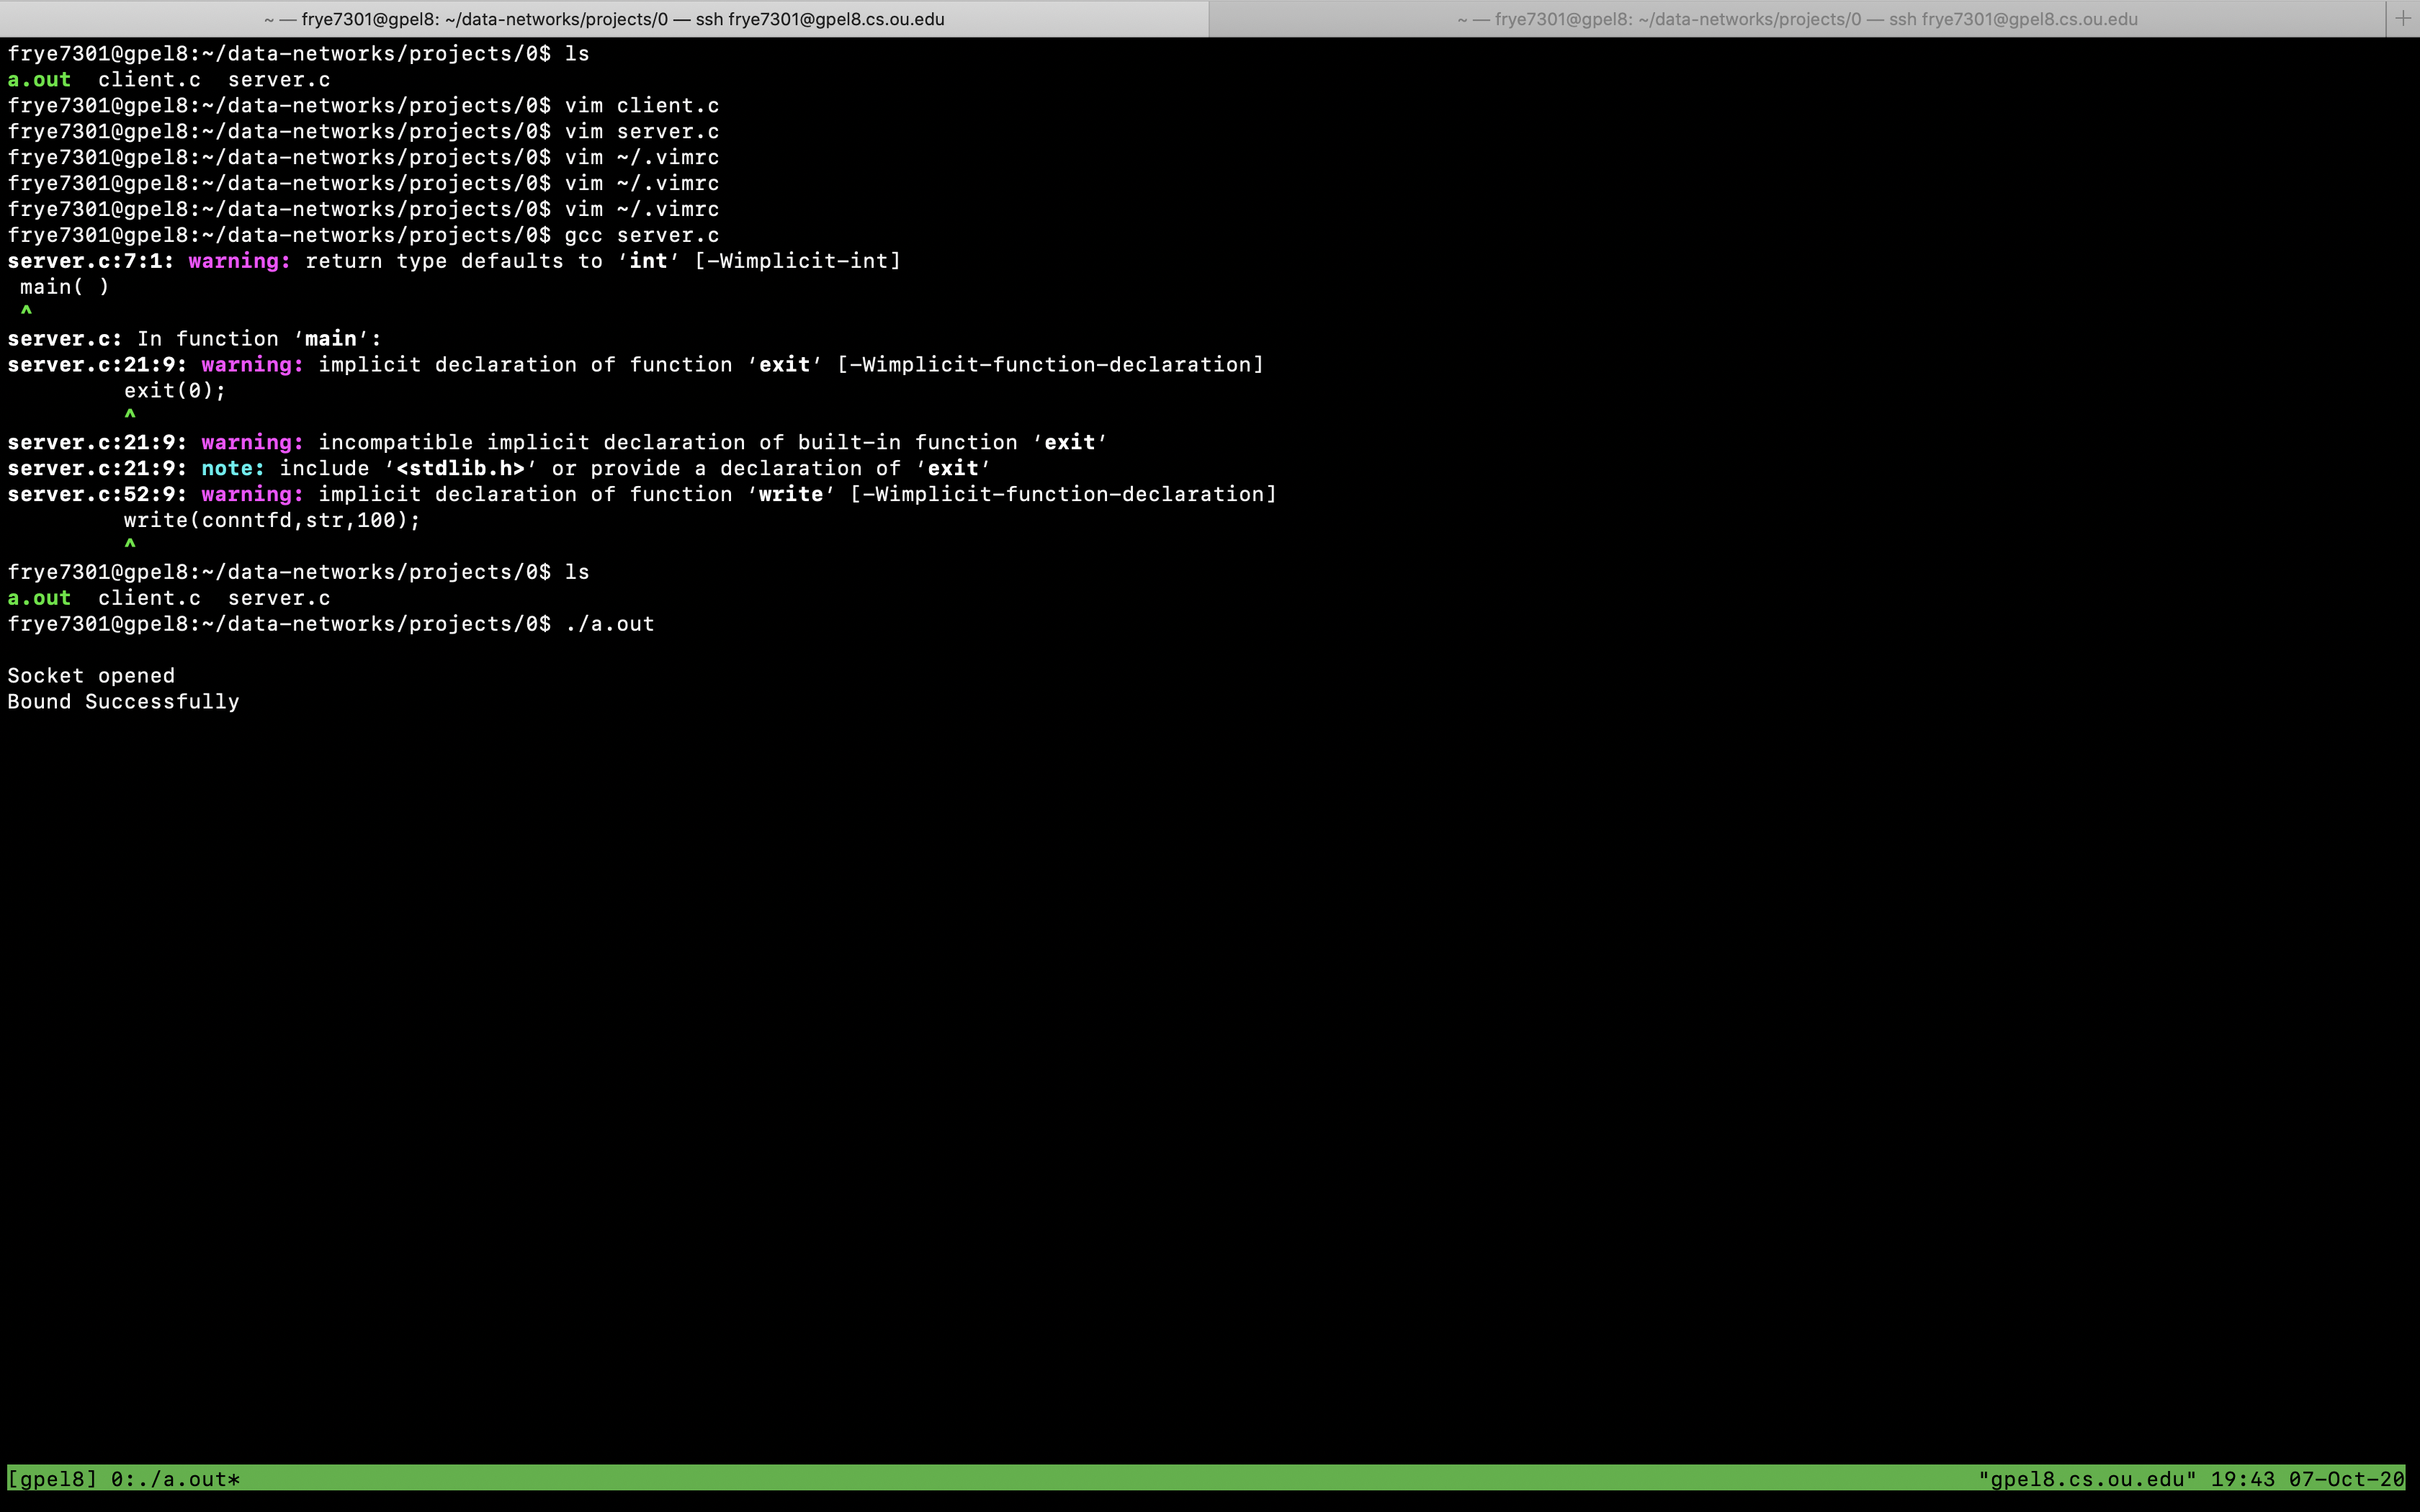
\includegraphics[scale=0.25]{server-client-local.png}
    
    \section*{Client Running on gpel8}
    
    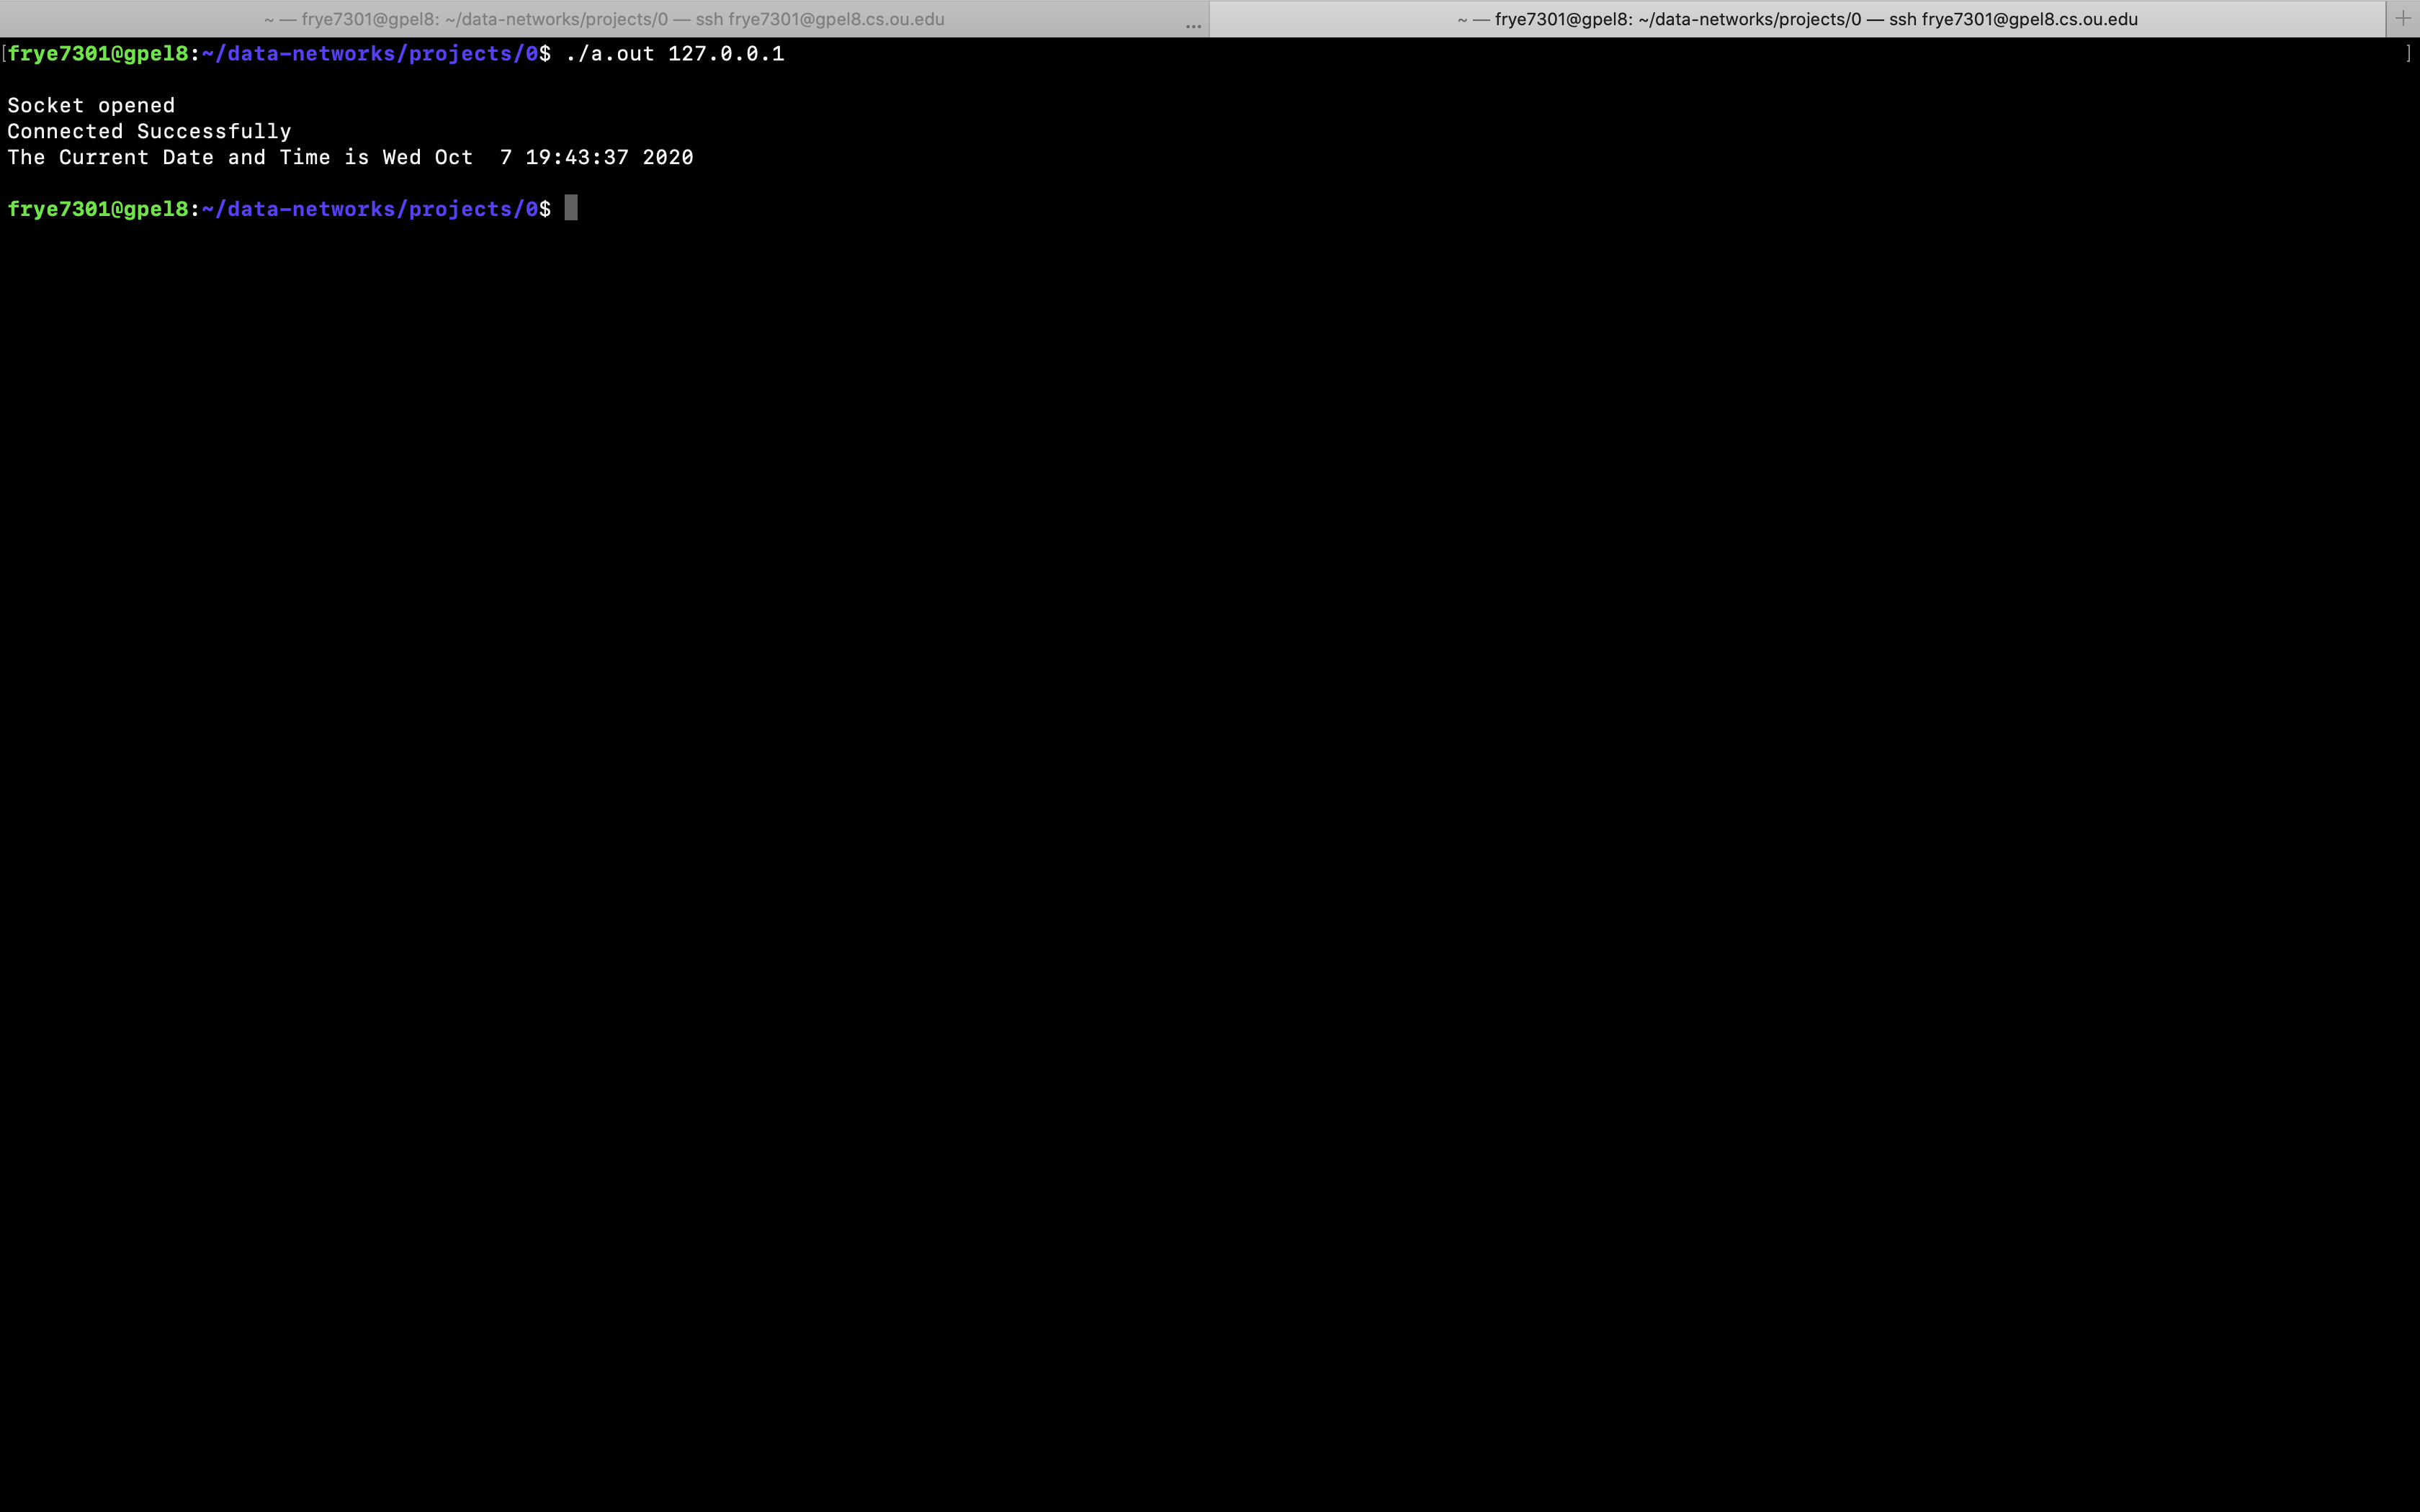
\includegraphics[scale=0.25]{client-server-local.png}

    \section*{Server running on gpel11 and Client on gpel8}

    To get this part working I copied the code over to gpel11, retrieved that machine's IP address, and then ran the server on it. On gpel8 I ran the client using gpel11's IP address as the input.
    
    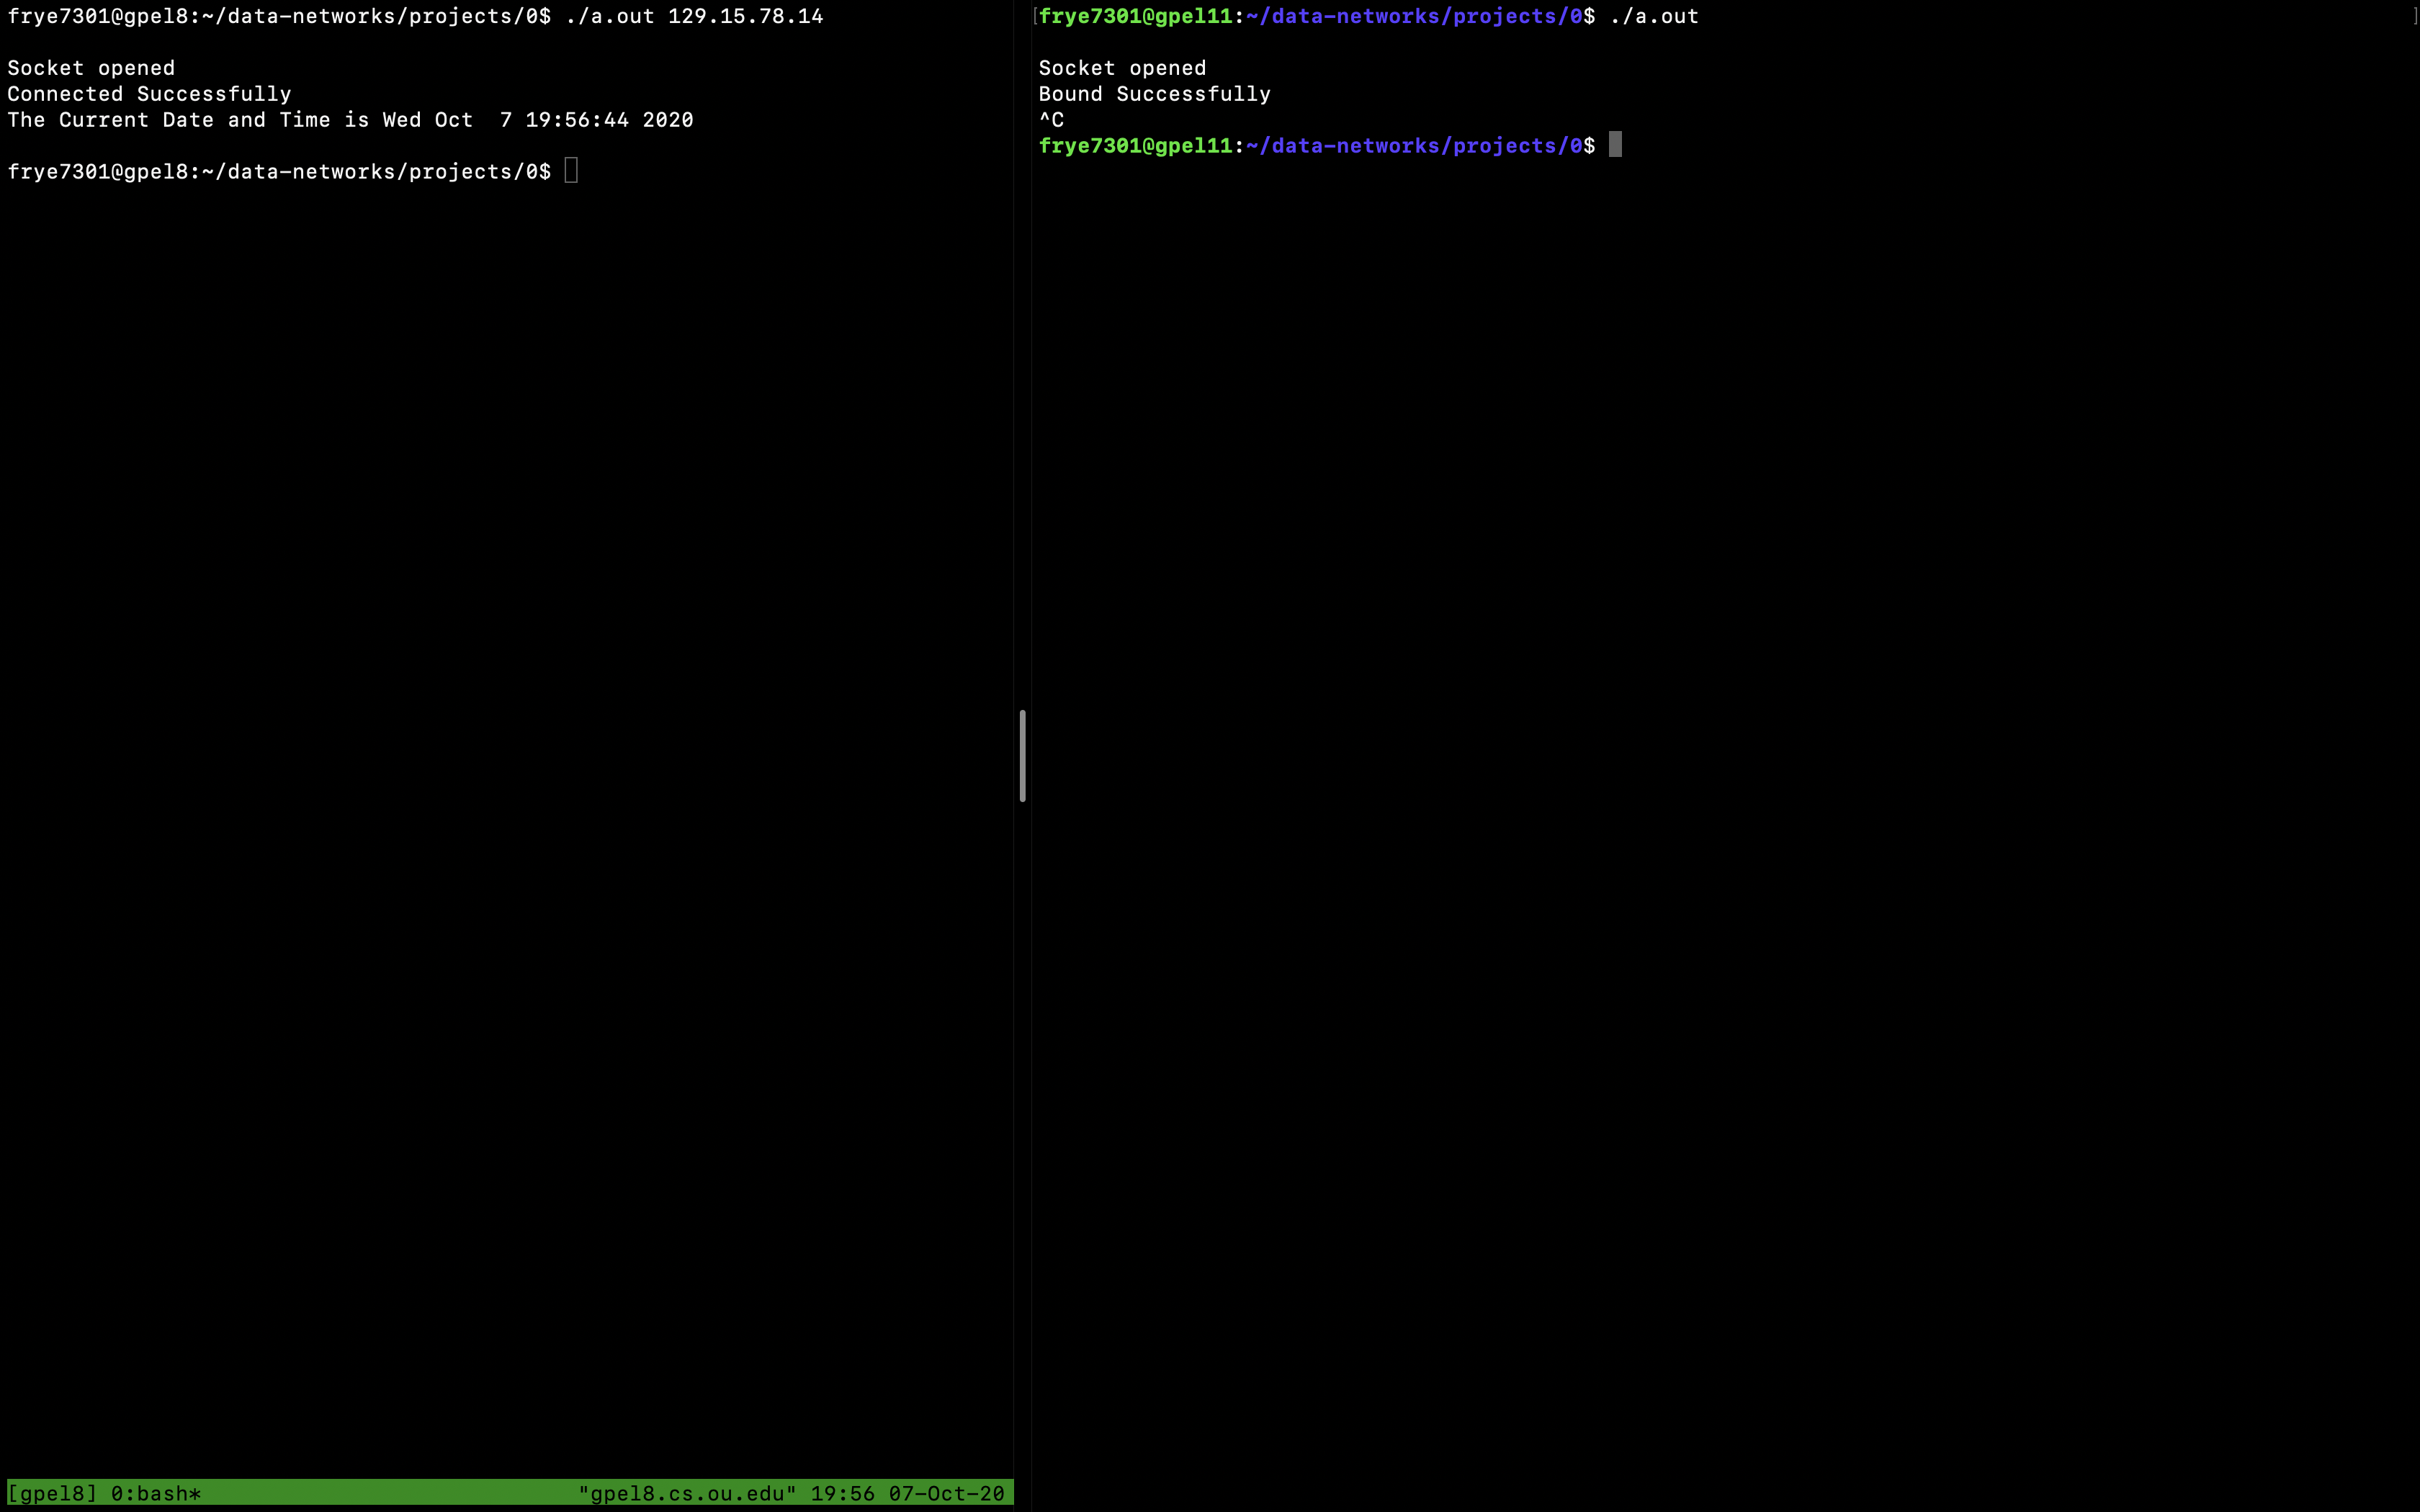
\includegraphics[scale=0.25]{client-server-across.png}
    

\end{document}
